\documentclass{article}

% if you need to pass options to natbib, use, e.g.:
%     \PassOptionsToPackage{numbers, compress}{natbib}
% before loading neurips_2020

% ready for submission
% \usepackage{neurips_2020}

% to compile a preprint version, e.g., for submission to arXiv, add add the
% [preprint] option:
%     \usepackage[preprint]{neurips_2020}

% to compile a camera-ready version, add the [final] option, e.g.:
    % \usepackage[final]{neurips_2020}

% to avoid loading the natbib package, add option nonatbib:
     \usepackage[final, nonatbib]{neurips_2020}

\usepackage[utf8]{inputenc} % allow utf-8 input
\usepackage[T1]{fontenc}    % use 8-bit T1 fonts
\usepackage{hyperref}       % hyperlinks
\usepackage{url}            % simple URL typesetting
\usepackage{booktabs}       % professional-quality tables
\usepackage{amsfonts}       % blackboard math symbols
\usepackage{nicefrac}       % compact symbols for 1/2, etc.
\usepackage{microtype}      % microtypography
\usepackage{float}
\usepackage{graphicx}
\usepackage{amsmath}

\newcommand{\del}{\partial}


\title{Interpolating Vector Fields with the Vector Heat Method}

% The \author macro works with any number of authors. There are two commands
% used to separate the names and addresses of multiple authors: \And and \AND.
%
% Using \And between authors leaves it to LaTeX to determine where to break the
% lines. Using \AND forces a line break at that point. So, if LaTeX puts 3 of 4
% authors names on the first line, and the last on the second line, try using
% \AND instead of \And before the third author name.

\author{
  Mark Nishimura \\  Stanford University
}

\begin{document}

\maketitle

% \begin{abstract}
%   asdf
% \end{abstract}

\section{Introduction}
The Vector Heat Method \cite{Sharp:2019:VHM} is a method for computing the
global parallel transport of vectors using heat diffusion, yielding fast and
efficient results.

In this report, we do the following:
\begin{itemize}
  \item We provide an implementation of the vector heat method for triangular meshes in Julia.
  \item We use the method to perform nearest-neighbor vector interpolation on a variety of shapes.
\end{itemize}

\section{Preliminaries}
\subsection{Scalar heat diffusion}
The heat equation describes the process of heat diffusing on a manifold $\mathcal{M}$ over time
\begin{equation}\label{eqn:heat}
  \frac{d}{dt}u(x,t) = \Delta u(x, t)
\end{equation}
where $\Delta = \nabla \cdot \nabla$ is the negative semidefinite
Laplace-Beltrami operator on $\mathcal{M}$. As a linear partial differential
equation, the solution after some time $t$ when $u(y, 0) = \delta_{x}(y)$ is given
by the heat kernel
\begin{equation}\label{eqn:scalarheatkernel}
  k_{t}(x, y) \sim C(x, y, t)j(x, y)^{-1/2} \left(1 + \sum_{i=1}^{\infty}t^{i}\Phi(x, y)\right).
\end{equation}
Here, $C$ is a constant and $j$ is a function of position, while $\Phi_{i}(x, y)$
are scalar-valued functions. As we will see soon when we consider vector heat diffusion, the exact structure of the
functions $j$ and $\Phi_{i}$ are not particularly important, but the particular
form of the kernel is.

\subsection{Parallel Transport}
Intuitively, the parallel transport of a vector $v$ on a manifold $\mathcal{M}$
along a path $\gamma_{a \to b}$ is the output of translating the vector along
$\gamma$ without ``tangential acceleration''. More formally the (extrinsic)
covariant derivative (if defined intrinsically, it is the Levi-Civita connection) of a vector field $Y$ along a basis direction $u^{i}$ is given by
\begin{equation}\label{eqn:covderiv}
  \nabla_{u^{i}}Y = \left[\frac{\del v^{k}}{\del u^{i}} + v^{j} \Gamma^{k}_{{ij}}\right]e_{k}
\end{equation}

\subsection{Vector diffusion}
Using the scalar heat equation as our guide, we define an analogous heat
equation for vector diffusion as follows:
\begin{equation}\label{eqn:vecheat}
  \frac{d}{dt}Y(x, t) = \Delta^{\nabla} Y(x, t)
\end{equation}
where this time, $Y$ is a vector. $\Delta^{\nabla}$ is called the
\textit{connection Laplacian} and is similarly defined to $\Delta$ as
$ \nabla \cdot \nabla $ where this time, $\nabla$ is the Levi-Civita connection.
This equation has a similar kernel solution
\begin{equation}\label{eqn:vectorheatkernel}
  k_{t}^{\nabla}(x, y) \sim C(x, y, t)j(x, y)^{-1/2} \left(\sum_{i=0}^{\infty}t^{i}\Psi_{i}(x, y)\right).
\end{equation}
Since convolution with the vector heat kernel must map a vector at
$x$ to vectors at all points $y$, the functions $\Psi_{i}(x, y)$ represent maps
from the space of vectors at $x$ to the space of vectors at $y$.

In particular, $\Psi_{0}(x, y) = P_{\gamma_{{x \to y}}}$, the parallel transport of $x$ to $y$
along the geodesic from $x$ to $y$. Noting that the coefficients $C$ and
functions $j$ are the same for both $\Delta$ and $\Delta^{\nabla}$, we see that
by diffusing the magnitudes of the vectors and the vectors themselves
separately, we can compute the vector parallel transport by dividing the two.
Furthermore, noting that nearest-neighbor scalar fields can be computed by
diffusing the point sources for short amounts of time and computing the average
value at each point, the authors consider the
following procedure. Given an initial configuration of vectors $Y_{0}$ with
magnitudes $u_{0}$ and support $\phi_{0}$
\begin{enumerate}
  \item Diffuse vectors $Y_{0}$ over the surface to get $Y_{t}$.
  \item Diffuse their magnitudes $u_{0}$ to get $u_{t}$.
  \item Diffuse indicator functions of the support $\phi_{0}$ to get $\phi_{t}$.
  \item Compute $\frac{Y_{t}}{|Y_{t}|} \cdot u_{t}/\phi_{t}$
\end{enumerate}
See section 4.1 of \cite{Sharp:2019:VHM} for a more detailed explanation.

\section{Method}
To apply the vector heat method to an oriented triangle mesh, we must discretize the
operators $\Delta$ and $\Delta^{\nabla}$. Then, a single backward-Euler pass
solves the equation at all vertices of the mesh simultaneously.
\subsection{Discretized Parallel Transport}
\begin{figure}[H]\label{fig:tangentspace}
  \centering
  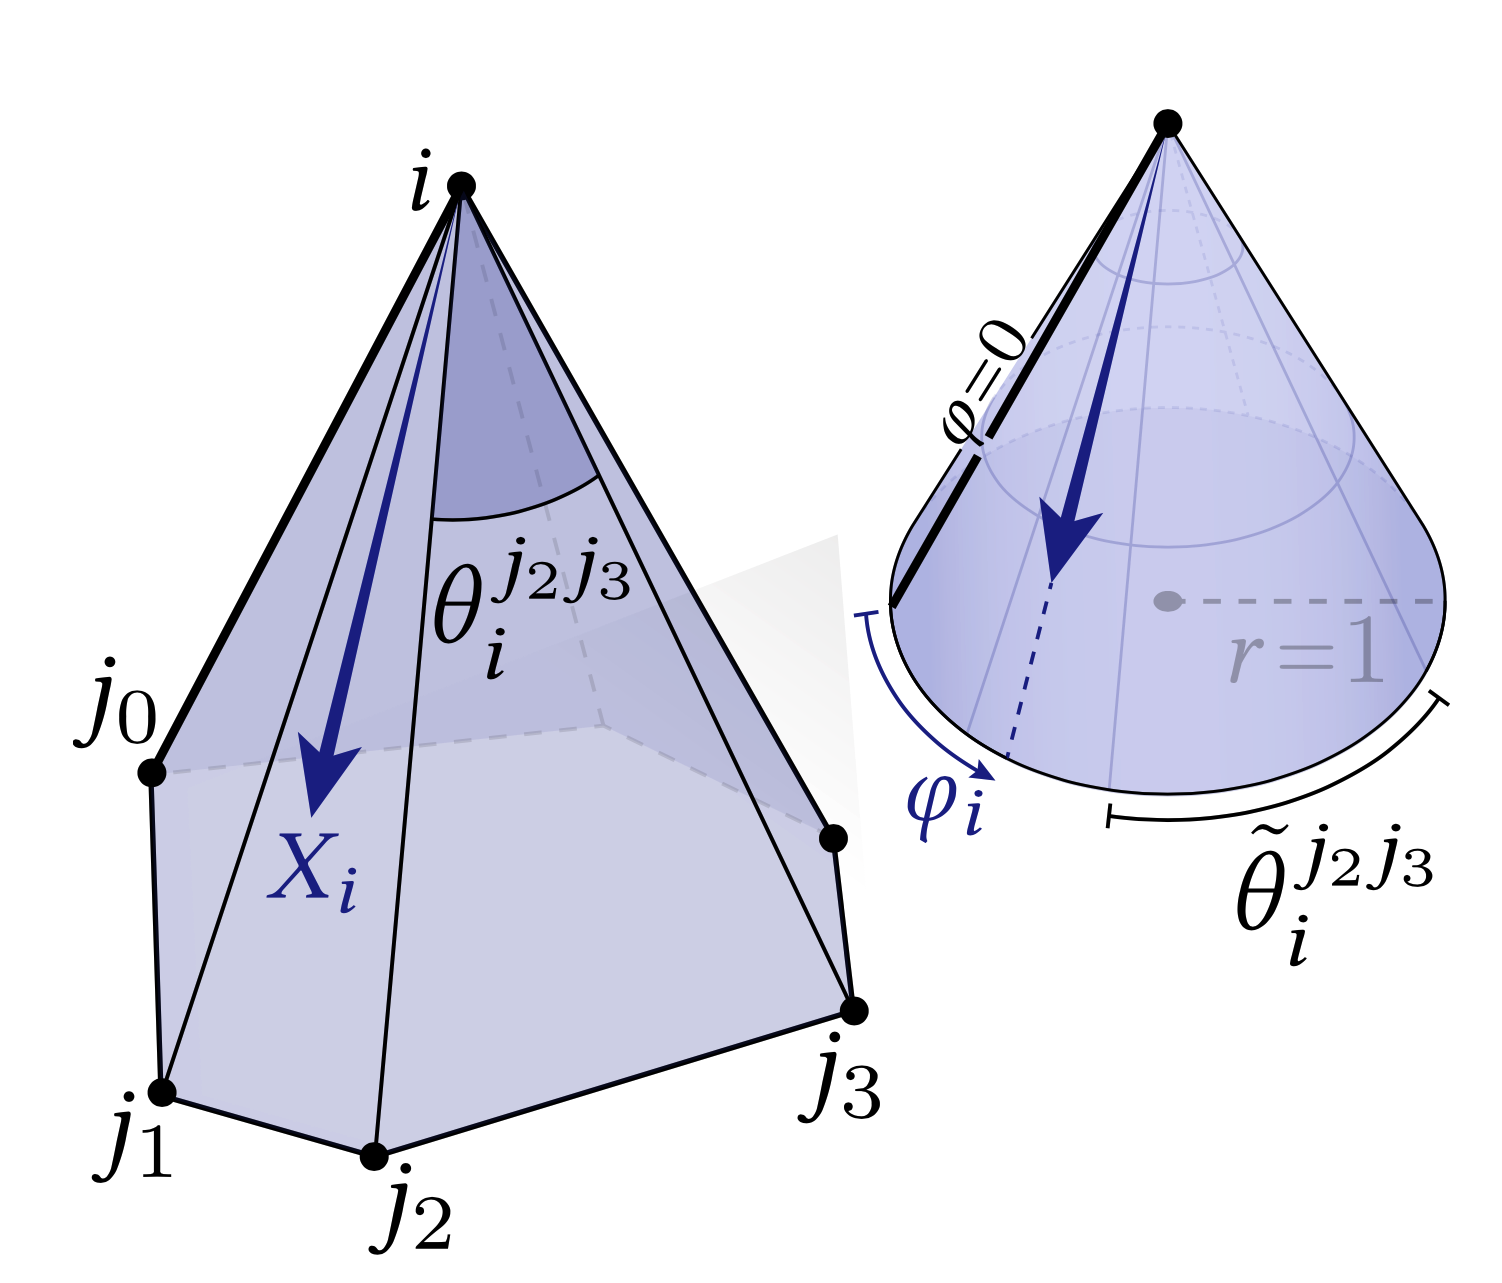
\includegraphics[height=5cm]{figures/tangentspace.png}
  \caption{Tangent space figure taken from \cite{Sharp:2019:VHM}. Vectors in
    the tangent space around vertex $i$ are represented as complex numbers with
    normalized angles $\theta$.}
\end{figure}
To compute the connection Laplacian, a notion of tangent space and parallel
tranport between mesh vertices is needed. The authors choose to use a normalized
angle approach. For every vertex, they pick a reference vertex $j_{0}$ and
arbitrarily set its angle to be $\phi = 0$. Going counter-clockwise around the
vertices and summing the inner angles $\theta^{j_{i}j_{{i+1}}}$ to get a total
inner angle $\Theta_{i}$. The normalized inner angles are then defined as
\begin{equation}\label{eqn:normangles}
  \tilde\theta_{i}^{jk} = 2\pi\theta_{i}^{{jk}}/\Theta_{i}
\end{equation}
and the angle of edge $ij_{a}$ is the cumulative sum
\begin{equation}\label{eqn:totalangles}
  \varphi_{ij_{a}} = \sum_{p=0}^{a-1}\tilde\theta_{i}^{j_{p}j_{p+1}}.
\end{equation}
Given these conventions, we note that a tangent vector with angle $0$ in
tangent space $T_{i}\mathcal{M}$ must be rotated by an angle equal to
$\varphi_{ji} + \pi - \varphi_{ij}$ to remain parallel in the tangent space
$T_{j}\mathcal{M}$ of an adjacent vertex $j$. Given this, we define rotation
constants $r_{ij}$ which are complex numbers describing how to parallel
transport vectors from the tangent space of $i$ to the tangent space of $j$.

\begin{equation}\label{rij}
  r_{ij} = e^{\imath(\varphi_{ji} + \pi - \varphi_{ij})}
\end{equation}
where $\imath$ is the imaginary unit $\imath^{2} = -1$.

\subsection{Solving for the Final Vector Fields}
To diffuse the vector fields, we first need the diagonal lumped mass matrix $M$
whose elements are the masses associated to each vertex (i.e. $1/3$ the area of
all adjacent triangles).
\begin{equation}\label{eqn:lumpedmass}
  M_{ii} = \sum_{{ijk} \in F} A_{ijk}.
\end{equation}

Given cotan weights $a = cot\theta_{i}^{jk}$, $b = cot\theta_{j}^{ki}$ and
$c = cot \theta_{k}^{ij}$, the matrix corresponding to the regular
Laplace-Beltrami operator $L$ multiplied by the mass matrix can be computed by
accumulating the following matrices into the appropriate entries of $L$:

\begin{equation}\label{eqn:laplacebeltrami}
  -\frac12 \cdot \left[
  \begin{array}{ccc}
    b + c & -c & -b \\
    -c & c + a & -a \\
    -b & -a & a+b
    \end{array}\right].
\end{equation}

The connection Laplacian $L^{\nabla}$ can be computed in the exact same way, but the relative
rotations between tangent spaces must be taken into account:
\begin{equation}\label{eqn:connectionlaplacian}
  -\frac12 \cdot \left[
  \begin{array}{ccc}
    b + c & -cr_{ji} & -br_{ki} \\
    -cr_{ij} & c + a & -ar_{kj} \\
    -br_{ik} & -ar_{jk} & a+b
    \end{array}\right].
\end{equation}
Note that this equation is actually different from the one in
\cite{Sharp:2019:VHM} - I suspect there is a typo.

Finally, we solve three linear systems to get the final answer (using
$t = (${average edge length}$)^{2}$ as a heuristic)
\begin{align*}
  (M - tL^{\nabla})Y &= Y_{0} \\
  (M - tL)u &= u_{0} \\
  (M - tL)\phi &= \phi_{0}
\end{align*}



\section{Results}
We implemented the Vector Heat Method in Julia. Some results for interpolating
vector fields are below.
\begin{figure}[H]\label{fig:sphere}
  \centering
  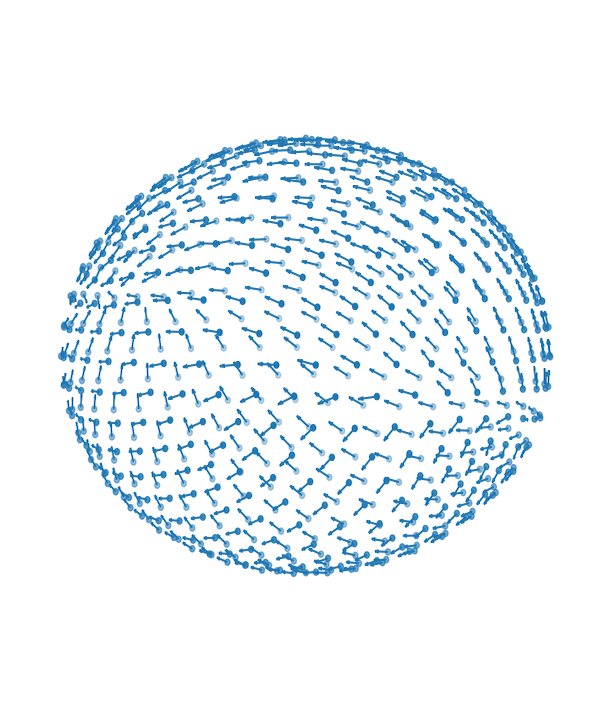
\includegraphics[width=0.5\textwidth]{figures/sphere.png}
  \caption{Running the vector interpolation method on a sphere with two separate
  initial points.}
\end{figure}

\begin{figure}[H]\label{fig:torus}
  \centering
  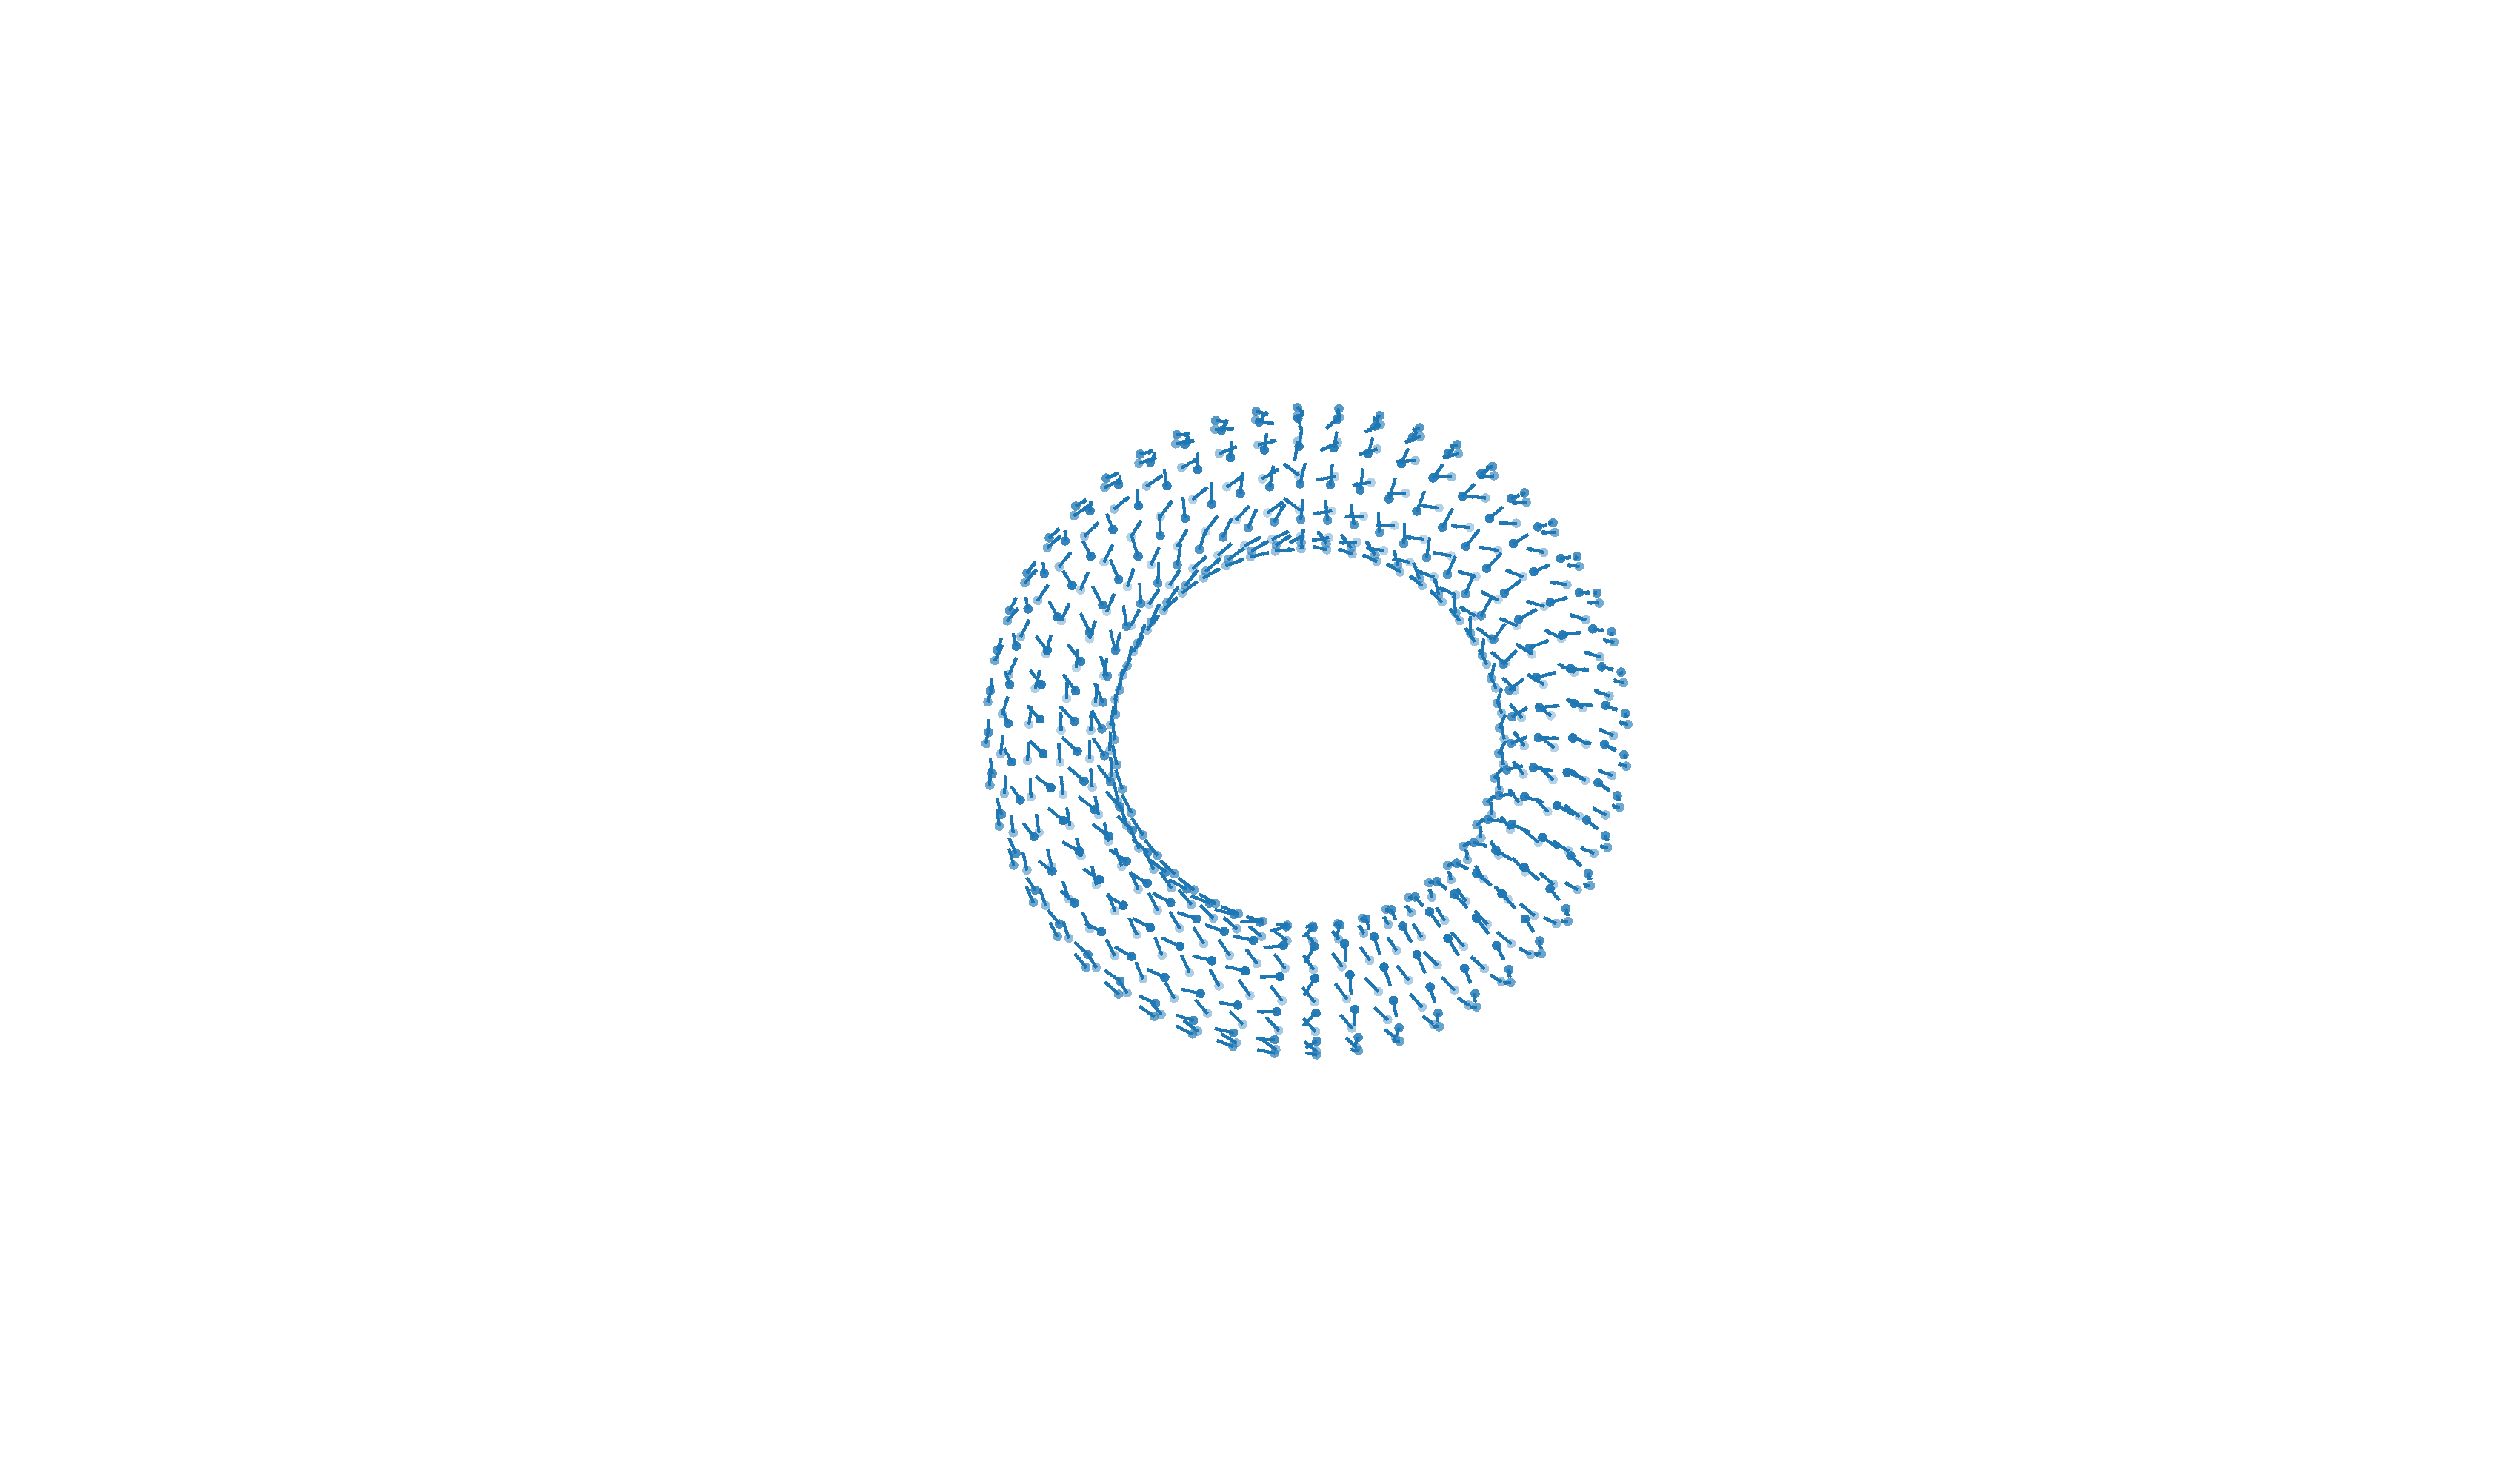
\includegraphics[width=0.5\textwidth]{figures/torus.pdf}
  \caption{Running the vector interpolation method on a torus with two separate
    initial points. The left-right separation between the two vector fields is }
\end{figure}

\section{Conclusion}
The ability to globally parallel transport vectors on meshes efficiently and
accurately opens up many possibilities for analyzing 3D geometry. For example,
transporting a (discretization of a) small ring of outward-pointing vectors,
results in a field that can be integrated to compute the logarithm map of a mesh.
The original authors also apply the vector
heat method to point clouds and voxelized representations, since the only thing
needed to compute the discrete laplace operators are distances and mappings
between local tangent spaces, neither of which are unique to triangle meshes.


\bibliographystyle{ieeetr}
\bibliography{refs}

\end{document}
